%mainfile: rapport.tex

\section{Interface graphique (IHM)}
\label{section:ihm}

\subsection{Présentation}

L'interface graphique permet l'utilisation de PIE par l'utilisateur local. Elle a pour vocation
de présenter une vue la plus complète possible de l'état de l'application à l'utilisateur, ceci
est réalisé à travers neuf onglets et une fenêtre. Un menu permet de changer l'état de l'application
et les vue (onglets/fenêtre) proposées. \\

\textbf{PIE's interface} : l'onglet principal, il offre une vue à l'utilisateur des flux disponible,
des flux auxquels l'utilisateur est abonné et une zone de texte afin que ce dernier puisse écrire et
envoyer des message (voir capture ci-dessous). Cet onlget est tout le temps ouvert. Il est possible
de s'abonner ou se désabonner d'un flux en le faisant glisser de la zone référençant les flux disponibles
vers celles référençant les flux auxquels l'utilisateur est abonné et vice-versa (drag and drop).\\

\begin{center}
    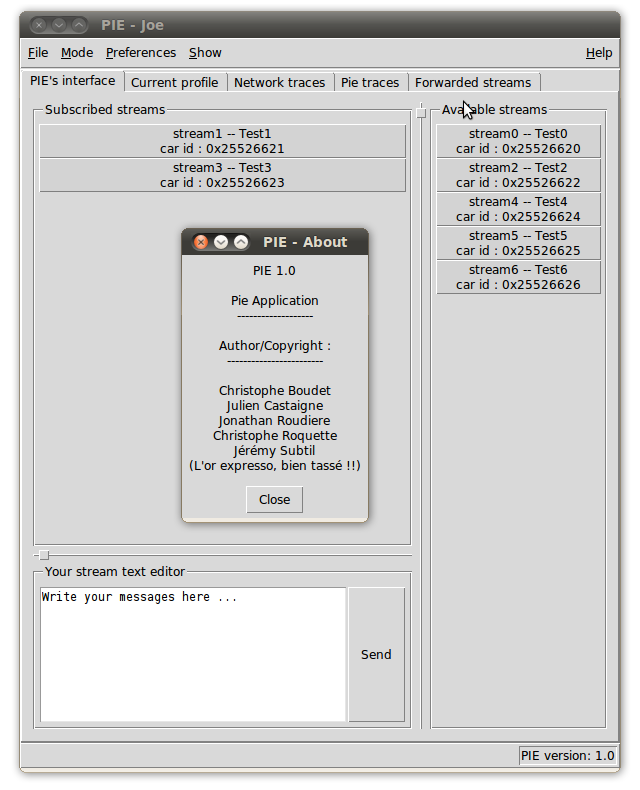
\includegraphics[width=0.9\textwidth]{img/pie-main.png}
\end{center}

\clearpage
\textbf{Current Profile} : onglet permet la consultation et la modification du profil de
courant de l'utilisateur local, si le profile est modifié il est alors enregistré. \\

\begin{center}
    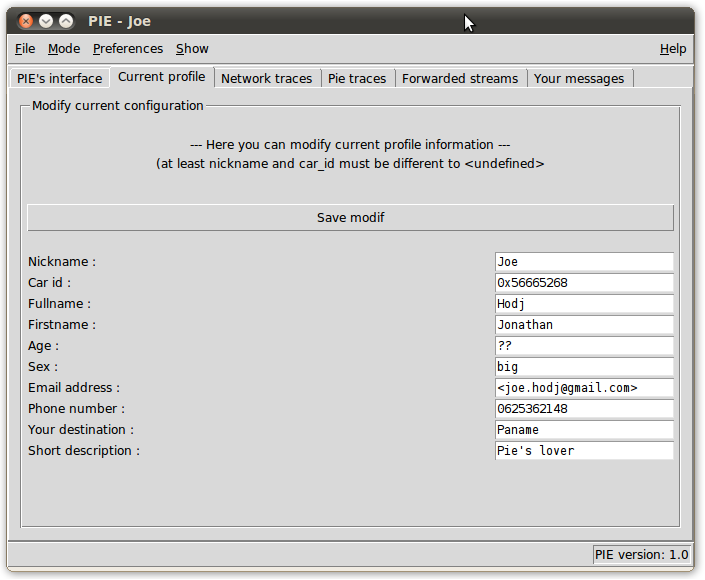
\includegraphics[width=0.9\textwidth]{img/profile.png}
\end{center}

\textbf{Global settings} : onglet permet la consultation et la modification des réglages 
d'ordre général de PIE (les onglets ouvert au démarage de l'application ou le mode par défaut). \\

\textbf{Your messages} : onglet qui permet de consulter les précédents messages envoyés par l'utilisateur local. \\

\textbf{Forwarded streams} : onglet qui permet de consulter les flux qui sont transmis à des paries, de mettre à jour 
les informations affichées et éventuellement d'arrèter la transmission de ce flux.\\

\begin{center}
    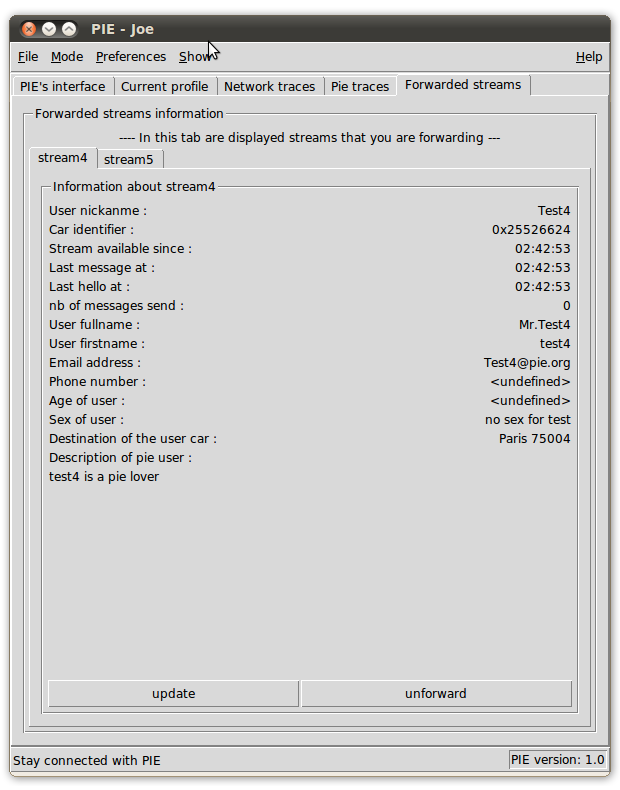
\includegraphics[width=0.9\textwidth]{img/forwarded.png}
\end{center}

\textbf{Subscribed streams} : fenêtre permettant de voir les flux auxquels l'utilisateur local est abonné, chaque flux est affiché dans un onlget,
les informations concernant le flux sont affichées ainsi que les messages qu'il a émis.\\

\begin{center}
    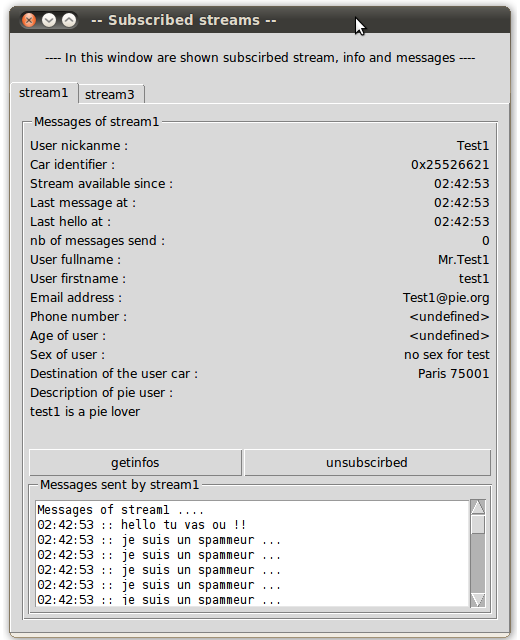
\includegraphics[width=0.9\textwidth]{img/subscribed.png}
\end{center}

\textbf{Pie traces} : onglet qui affiche toutes les traces (debug) de l'application et de ses sous-systèmes.\\

\textbf{Network traces} : onlget qui permet de consulter l'ensemble des messages émis ou reçus depuis le réseau dans leur forme brute.\\

\textbf{Input/Output traces} : deux onlget qui permettent de consulter l'ensemble des messages reçu/émis depuis le réseau dans leur forme brute. \\

\section{Compte utilisateur et configuration}

PIE utilise deux fichiers de configuration, le premier est celui définissant le profil de l'utilisateur
alors que le second permet de configurer l'application elle même (onlget ouvert, mode, ...).  \\

Les fichiers de configuration sont conservés dans le répertoire \textbf{\$HOME/.pie} (par défaut), le fichier
de configuration global doit s'appeler \textbf{global.conf} et les fichiers de profil utilisateur doivent
s'appeler \textbf{NICKNAME.conf}. \\

A son lancement l'interface graphique vérifie à travers le sous-système de gestion des configurations
que le répertoire de configuration et les fichiers précités sont présents, si ce n'est pas la cas alors le
répertoire de configuration et un fichier de configuration globale générique sont alors crées, l'utilisateur lui
est invité à définir un profil via l'IHM. \\

Si plusieurs profils utilisateur sont disponible alors l'utilisateur est invité à en choisir un. Une fois ces
vérifications faites et un profile déterminé l'application PIE est prête à être utilisée.

